%%%%%%%%%%%%%%%%%%%%%%%%%%%%%%%%%%%%%%%%%%%%%%%%%%%%%%%%%%
%%
%% MARK: Title & Data
%%
%%%%%%%%%%%%%%%%%%%%%%%%%%%%%%%%%%%%%%%%%%%%%%%%%%%%%%%%%%

\chapter*{\S B32. Lagrange's Equations of Motion}%
\setcounter{footnote}{0}

%%%%%%%%%%%%%%%%%%%%%%%%%%%%%%%%%%%%%%%%%%%%%%%%%%%%%%%%%%
%%
%% MARK: Abstract
%%
%%%%%%%%%%%%%%%%%%%%%%%%%%%%%%%%%%%%%%%%%%%%%%%%%%%%%%%%%%

\begin{abstract}
  In this note%
  \footnote{A piece included in a wider project: "The Geometry of {Motion}" a book to be published by the Beijing WPC.}
  I apply the Lagrange method of variation of constants to Newton's equations,
  by considering the force involved in the motion of a point as a perturbation of the absence of forces.
\end{abstract}

%%%%%%%%%%%%%%%%%%%%%%%%%%%%%%%%%%%%%%%%%%%%%%%%%%%%%%%%%%
%%
%% MARK: Content
%%
%%%%%%%%%%%%%%%%%%%%%%%%%%%%%%%%%%%%%%%%%%%%%%%%%%%%%%%%%%

This note should be seen as a \emph{Récréation},
a break from abstract diffeology to return to the physics for which diffeology was specifically developed.
It is not that diffeology is used in this note,
which is a reflection on Lagrange's equations of motion,
in relation to what is usually called the ``Hamiltonian formalism'',
but I hope that one day, in the near future, I will have some examples where this is the case.

In a paper on Lagrange's work
I explained how Lagrange introduced
the first elements of symplectic geometry when he applied
his {\em method of variation of constants} to the motion
of the Earth around the Sun, see
\cite{Lag08,Lag09,Lag10}.
In these memoirs, Lagrange regarded the motion of the Earth as a curve in
the space of its Keplerian elements, the points of the curve representing,
at each time, the Keplerian motion that the Earth would follow if the forces
exerted by the other planets ceased at that instant.
The motion of the planet is then described not in space-time but in
the {\em space of Keplerian motions}, that is, by the curve of its
{\em tangential Keplerian motions}
at each instant. The question then consists
in expressing the differential equation satisfied by this curve and eventually
in extracting
some information on the stability of the system.
It was when he established the nature of this curve that Lagrange introduced his
{\em system of parentheses} which constitute
the coordinates of the --- today canonical --- {\em symplectic structure}
on the space of Keplerian motions.
It was the birth of symplectic calculus and then symplectic geometry,
see \cite{PIZ98,PIZ02}.

But Lagrange's method of variation of constants applies
in the first place to the basic Newton's equations where the force
applied to a point is measured by the
deflection of the tangential {\em inertial motion} (see Figure \ref{tangent-motion}).
The motion of the point is then regarded as a
curve in the space of its tangent inertial motions,
for which we shall establish the
differential equation.
That is the original Lagrange interpretation of Newton's equations,
an idea fully contained, but implicitly, in his second paper on the question
in 1809, {\em op. cit.}
I shall give in the following a modern construction of these {\em Lagrange equations of motion}.

\Note A physicist would say that the construction below is
just a change of variables.%
\footnote{That is what happened to me during a talk at IHES.}
It may appear that way at first glance, but on a conceptual level,
it does not reduce to just that.
Newton's equations are by construction Aristotelian:
they assume not only an absolute time --- which is acceptable at this
epoch --- but also an absolute space, since Newton's equations are all
about the second variation of
position in space. Meanwhile, since Galileo, we know that there is
no such space, or if you prefer,
there is no mechanical way, in the world we live in, to distinguish a
rectilinear uniform motion from rest.%
\footnote{As a first approximation,
of course, reality being more complex.}
Thus, Newton's equations, as they are taught in school,
are not even compatible with Galilean principles,%
\footnote{This is what
generates so much confusion in school textbooks about Newton's equations.}
but they are still not too far.
We shall see how the Lagrange point of view
transforms the Aristotelian Newton's equations into a system respectful
of Galilean relativity.

%%%%%%%%%%%%%%%%%%%%%%%%%%%%%%%%%%%%%%%%%%%%%%%%%%%%%%%%%%
%%
%% MARK: The space of inertial motions
%%
%%%%%%%%%%%%%%%%%%%%%%%%%%%%%%%%%%%%%%%%%%%%%%%%%%%%%%%%%%
\section{The space of inertial motions}

First of all, let us build the space of inertial motions on which we will
draw the curve representing the motion of our system.
Considering the simple case of a free particle in $\RR^3$, an inertial motion
is just a uniform rectilinear motion, that is, a curve
$$
  \mu = [t \mapsto x(t)] \quad \text{such that} \quad {d^2x \over dt^2} = 0.
$$
Let us denote by $\cM_0$ this space of uniform rectilinear motions.
$\cM_0$ is a smooth manifold
and we have a particular global chart:
$$
  \Phi : \RR^3 \times \RR^3 \to \cM_0, \quad \Phi(x,v) = [t \mapsto x + tv].
$$
Now, let us consider the motion of a particle of mass $m$ subjected to a
force $F$, that is, a curve $t \mapsto x(t)$ in $\RR^3$ satisfying
Newton's equation:
$$
  m {d^2x(t) \over dt^2} = F(x(t),t).
$$
The force $F$ is assumed to be a smooth function defined on (an open subset of) $\RR^3 \times \RR$.
At each instant $t$ we can define the {\em tangent inertial motion} to the
motion $[t \mapsto x(t)]$ as the uniform rectilinear motion $\mu(t)$ passing through
$x(t)$ at time $t$, with velocity $v(t)= dx(t)/dt$, that is,
$$
  \mu(t) = [s \mapsto x(t) - t v(t) + s v(t)].
$$
In other words, \uline{the tangent inertial motion at instant $t$ is the inertial motion that
the particle would follow if the force vanished at that instant}.

%%###########
\begin{figure}[th]
  \centerline{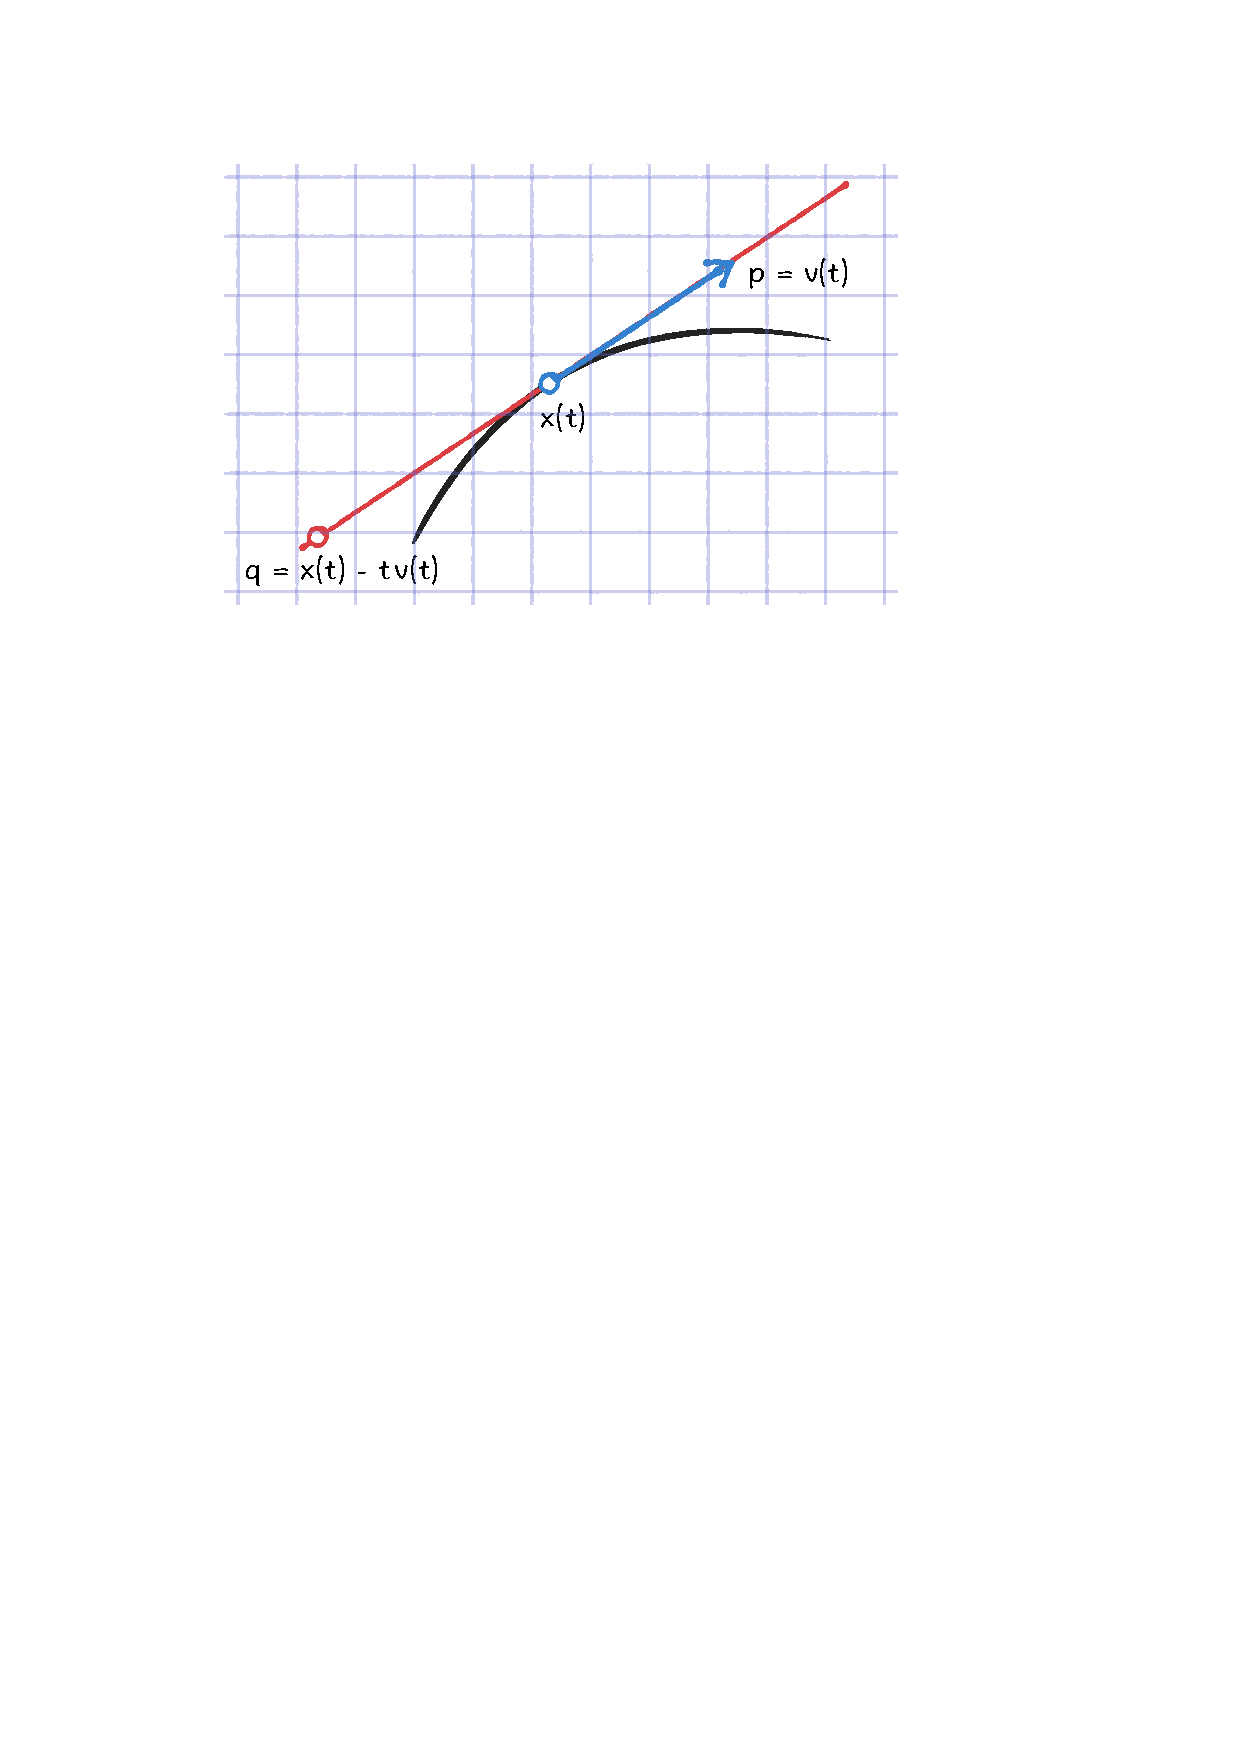
\includegraphics[width=0.66\textwidth]{Figures/TangentMotion.pdf}}
  \caption{Tangent inertial motion.}
  \label{tangent-motion}
\end{figure}
%%###########

Hence, the curve $t \mapsto \mu(t)$ represents the motion of the particle,
but drawn in the space of inertial motions. Let us now determine the differential
equation that this curve satisfies. We shall follow Lagrange's hypothesis that
there exists a {\em potential} $\Omega$ for the force, that is,
$$
  F(x,t) = -{\partial \Omega(x,t) \over \partial x}.
$$
In the chart $\Phi$, the curve $t\mapsto \mu(t)$ becomes:
$$
  \mu(t) = \Phi(q(t),p(t)) \quad \text{with} \quad
  \left\{
  \begin{array}{rcl}
  q(t) & = & x(t) - t v(t), \\
  p(t) & = & v(t).
  \end{array}
  \right.
$$
This gives the differential system
\begin{eqnarray*}
  {dq(t) \over dt} & = & {dx(t) \over dt} - v(t) - t{dv(t) \over dt} = -t{dv(t) \over dt},\\
  {dp(t) \over dt} & = & {dv(t) \over dt}.
\end{eqnarray*}
Now, since the map $(x,v,t) \mapsto (q=x-tv,\; p=v,\; t)$ is a diffeomorphism, the potential
$\Omega$ can be written indifferently as a function of $(x,v,t)$ or $(q,p,t)$.
From the relations between partial derivatives:
\begin{eqnarray*}
  {\partial \Omega \over \partial q} & = & {\partial \Omega \over \partial x}{\partial x \over \partial q}
  + {\partial \Omega \over \partial v}{\partial v \over \partial q}
  + {\partial \Omega \over \partial t}{\partial t \over \partial q}, \\
  {\partial \Omega \over \partial p} & = & {\partial \Omega \over \partial x}{\partial x \over \partial p}
  + {\partial \Omega \over \partial v}{\partial v \over \partial p}
  + {\partial \Omega \over \partial t}{\partial t \over \partial p},
\end{eqnarray*}
with $x = q + tp$, $v = p$, and noting that, by hypothesis,
$\Omega$ does not depend on $v$, we eventually obtain
$$
  {\partial \Omega \over \partial q} =  {\partial \Omega \over \partial x}
  \quad \text{and} \quad
  {\partial \Omega \over \partial p} = t {\partial \Omega \over \partial x},
$$
which gives
$$ \renewcommand{\arraystretch}{2}
  \begin{array}{rclcccccl}
  \displaystyle {dq(t) \over dt} & = & \displaystyle -t{dv(t) \over dt} & = & \displaystyle - {t\over m}F(x(t),t) & = & \displaystyle  + {t \over m} {\partial \Omega \over \partial x} & = & \displaystyle  + {1 \over m} {\partial \Omega \over \partial p} \\[1ex]
  \displaystyle {dp(t) \over dt} & = & \displaystyle \phantom{-t}{dv(t) \over dt} & = & \displaystyle +{1\over m}F(x(t),t) & = & \displaystyle - {1 \over m} {\partial \Omega \over \partial x} & = & \displaystyle - {1 \over m} {\partial \Omega \over \partial q}.
  \end{array}
$$
Now, if we consider the symplectic structure defined on $\cM_0$,
in the chart $\Phi$, by
\renewcommand{\theequation}{$\clubsuit$}
\begin{equation}
  \omega(\delta \mu,\delta'\mu) = m\left[\langle \delta v,\delta' x\rangle -
  \langle \delta' v,\delta x\rangle\right] \quad \text{with} \quad \mu = \Phi(x,v),
\end{equation}
we recognize in the differential system above the symplectic gradient of
the potential $\Omega$. Newton's equations then become:
\renewcommand{\theequation}{$L$}
\begin{equation}
  {d \mu(t) \over dt} = \grad(\Omega).
\end{equation}
We recall that the symplectic gradient of a real function $f$ is defined by the identity
$$
  \grad(f) = - \DForms^{-1}(df) \quad \text{or} \quad
  \omega(\grad f,\delta \mu) = -df(\delta \mu),
$$
for all $\delta \mu \in \Tgt_\mu(\cM_0)$.
Equations $(L)$ are the {\em Lagrange equations of motion}. They
are exactly described in Lagrange's second memoir of 1809, on the
method of variation of constants in all problems of mechanics \cite{Lag09};
only the notations differ.
Their construction leads to a few remarks:

\Note{1.} Lagrange's equations of motion respect Galilean relativity:
the Galilean group acts naturally (by construction) on the space of inertial motions
$\cM_0$; that is, every element $g$ of the Galilean group transforms an inertial motion
$\mu$ into another inertial motion $g_*(\mu) = g \circ \mu$. Moreover, the Galilean group
preserves the symplectic structure on $\cM_0$, $g^*(\omega) = \omega$,
and the nature of equations $(L)$ is preserved under
a Galilean transformation. Precisely, for a curve $t \mapsto \mu(t)$ satisfying
equations $(L)$, the curve $g_*(\mu)$ satisfies
$$
  {d[g_*(\mu)](t) \over dt} = \grad(g_*(\Omega)),
$$
where $g_*(\Omega) = \Omega \circ g^{-1}$.
Thus, Lagrange's version of Newton's equations
behaves correctly with respect to Galilean relativity.

\Note{2.} The term $\grad(\Omega)$ in the equations above represents literally the force
exerted on the point in this covariant Lagrange symplectic framework.
It is a well-defined geometrical object, and the
Lagrange equations of motion state the obvious, since Galileo:
\uline{the force exerted on a particle is measured by the variation
of the inertial motion}.
If the force vanishes then $\mu = \text{const}$, \emph{i.e.}, in the absence of force the particle
follows an inertial motion.

\Note{3.} Lagrange's equations of motion look like Hamilton's equations,
but they are not exactly the same.
Indeed,
Hamilton's equations involve the whole Hamiltonian $H = p^2 / 2m + \Omega$ and not only the potential $\Omega$,
as is the case in Lagrange's equations.
In the Hamiltonian framework,
the space involved is not regarded as the space of inertial motions
(which is by construction Galilean-respecting)
but rather as the space of initial conditions at some instant $t_0$, a {\em phase space}
(which is not Galilean-respecting for the reason evoked above). This should also be seen in the light of what Souriau
wrote in the introduction of his book ``Structure des Systèmes Dynamiques'' \cite{Sou70}:

\begin{quote}``La mécanique analytique n'est pas une théorie périmée; mais
  il apparaît que les catégories qu'on lui attribue classiquement :
  {\em espace de configuration}, {\em espace de phases}, {\em formalisme lagrangien},
  {\em formalisme hamiltonien}, le sont ; ceci simplement parce qu'elles ne
  possèdent pas la covariance requise; en d'autres termes, parce
  qu'elles sont en contradiction avec la {\em relativité galiléenne}\dots''.%
  \footnote{Free translation: ``Analytical mechanics is not an outdated theory;
  but it appears that the categories classically attributed to it:
  configuration space,
  phase space,
  Lagrangian formalism,
  Hamiltonian formalism,
  are (outdated);
  this is simply because they do not possess the required covariance;
  in other words,
  because they are in contradiction with Galilean relativity\dots''
  }
\end{quote}

With Lagrange's method, in comparison with the usual Hamiltonian formalism,
the purely kinetic term of the Hamiltonian $p^2/2m$ is absorbed into the manifold of inertial motions
and its symplectic structure. That is why Newton's equations, in the above form $(L)$,
involve only the potential of the external force.

\Note{4.} Now it is easy to imagine more sophisticated situations, for example considering geodesics
of the sphere as inertial motions, or the original Lagrange construction with
Keplerian motions as inertial motions, etc. This Lagrange approach solves the question of equivariance
of the dynamics by avoiding reference to configuration or phase spaces, except perhaps in
the preliminary construction of the inertial motions which are at the foundation
of the method.

%%%%%%%%%%%%%%%%%%%%%%%%%%%%%%%%%%%%%%%%%%%%%%%%%%%%%%%%%%
%%
%% MARK: Deployment of the perturbation
%%
%%%%%%%%%%%%%%%%%%%%%%%%%%%%%%%%%%%%%%%%%%%%%%%%%%%%%%%%%%
\section{Deployment of the perturbation}

One can deploy the perturbation along time, that is, consider a new dynamical system
defined by a presymplectic structure $\omega$ on $\cY = \cM_0 \times \RR$, with
$$
  \omega = \omega_0 \ominus d[\Omega dt] = \omega_0 \ominus d\Omega \wedge dt,
$$
where $\omega_0$ now denotes the symplectic form on the space $\cM_0$ of inertial motions.
Let $y = (\mu,t)$ be a current point in $\cY$ with $\delta y$ and $\delta'y$ in
$T_y(\cY) = \Tgt_\mu(\cM_0) \times T_t(\RR)$. The evaluation of $\omega$ becomes:
\begin{eqnarray*}
  \omega(\delta y, \delta'y) & = & \omega_0(\delta \mu,\delta'\mu) -
  d\Omega(\delta \mu) \delta't + d\Omega(\delta'\mu)\delta t \\
  & = & \omega_0(\delta \mu,\delta'\mu) + \omega_0(\grad(\Omega)\delta't,\delta \mu)\\
  & - & \omega_0(\grad(\Omega)\delta t,\delta'\mu) \\
  & = & \omega_0(\delta \mu - \grad(\Omega)\delta t, \delta' \mu - \grad(\Omega)\delta' t).
\end{eqnarray*}
The $2$-form $\omega$ on $\cY$ is clearly presymplectic;
its kernel is
$1$-dimensional and given by:
$$
  \ker(\omega_y)= \{\delta y \in T_y(\cY) \mid \delta \mu = \grad(\Omega)\delta t\}.
$$
The point to clarify here is the meaning of $\grad(\Omega)$. First of all,
the potential $\Omega$
is a function of $y = (\mu,t)$, as we have seen. Then at the point $y = (\mu,t)$,
$\grad(\Omega)$ denotes the gradient, with respect to $\omega_0$, of the
function $\mu \mapsto \Omega(\mu,t)$ defined on $\cM_0$. We find here
a version of Souriau's construction of the space of motions of a dynamical system
\cite{Sou70}, but built over the inertial motions instead of built on a phase space.

Now, the quotient of $\cY$ by the characteristic foliation of $\omega$ is a smooth manifold
$\cM$. Indeed, the distribution $y \mapsto \ker(\omega_y)$ is transverse to the
slices $\cM_0 \times \{t\}$, and the restrictions $\pi_t$ of the projection $\pi : \cY \to \cM$ to
$\cM_0 \times \{t\}$ form an atlas of $\cM$. Moreover, since $\omega$ is closed,
denoting by $\xi$ the vector field
$\xi(y) = (\grad(\Omega),1)$ generating $\ker(\omega_y)$, we get
$\DLie_\xi(\omega) = 0$, which implies that there exists a closed $2$-form,
denoted by the same letter
$\omega$, on $\cM$ such that its pullback to $\cY$ by $\pi$ is $\omega$. Of course,
if the characteristic flow $\xi$ is complete, that is, if the second projection
$\Proj_2 : \cY \to \RR$, restricted to every integral curve, is surjective, then
$(\cM,\omega)$ is symplectomorphic to $(\cM_0,\omega_0)$.

%%%%%%%%%%%%%%%%%%%%%%%%%%%%%%%%%%%%%%%%%%%%%%%%%%%%%%%%%%
%%
%% MARK: Example of the oscillator
%%
%%%%%%%%%%%%%%%%%%%%%%%%%%%%%%%%%%%%%%%%%%%%%%%%%%%%%%%%%%
\section{Example of the oscillator}

We consider a pair of points $x = (x_1,x_2) \in \RR^3 \times \RR^3$ and the
Newton's equations
$$
  {d^2 x(t) \over dt^2} = \begin{pmatrix} x_2(t) - x_1(t) \\ x_1(t) - x_2(t) \end{pmatrix}.
$$

(A) {\bf The symplectic form on inertial motions.} ---
A variation of an inertial motion $\mu \in \cM_0$ necessarily has the form
$$
  \delta \mu = [t \mapsto \delta X + t \delta v] \in \Tgt_\mu(\cM_0).
$$
Denoting by $\dot \mu$ the velocity
of the motion we can check that, for two such variations $\delta \mu$ and
$\delta' \mu$, the value
\renewcommand{\theequation}{$\spadesuit$}
\begin{equation}
  \omega(\delta\mu,\delta'\mu) = m\left[\langle \delta \dot \mu(t),\delta'\mu(t)\rangle -
  \langle \delta'\dot\mu(t),\delta \mu(t)\rangle\right]
\end{equation}
does not depend on the instant $t$ at which it is computed, and it is equal to the
expression given in $(\clubsuit)$ above.

(B) {\bf The action of the Galilean group.} ---
The action of the Galilean group assumes a space-time $E = \RR^3 \times \RR$;
the points of $E$ are denoted by $(x,t)$. The Galilean group is the following
group of matrices, with $A \in \SO(3)$, $b,c \in \RR^3$ and $e \in \RR$:
$$
  g =
  \begin{pmatrix}
  A & b & c \\
  0 & 1 & e \\
  0 & 0 & 1
  \end{pmatrix} \quad \text{and} \quad 
  \begin{pmatrix}
  A & b & c \\
  0 & 1 & e \\
  0 & 0 & 1
  \end{pmatrix} \begin{pmatrix} x \\ t \\ 1 \end{pmatrix} =
  \begin{pmatrix} A x + bt + c \\ t+e \\ 1 \end{pmatrix},
$$
where $E$ is embedded in this affine picture as the level $1$ of $E \times \RR$.
Now, an inertial motion is an affine line in $E$, that is:
$$
  \mu = \left\{\begin{pmatrix}x + tv \\ t\end{pmatrix} \in E \mid t\in \RR \right\},
$$
where, as usual, $x,v \in \RR^3$. Then, the Galilean group acting on $E$ maps the affine line
$\mu$ into another affine line $g(\mu)$, and immediately:
$$
  g(\mu) = \left\{\begin{pmatrix}A x + c + t(A v + b) \\ t + e
  \end{pmatrix} \in E \mid t\in \RR \right\},
$$
or again:
$$
  g(\mu) = [t \mapsto A x + c + (t-e)(A v + b)].
$$
The symplectic form $\omega$ on $\cM_0$ is obviously invariant under $g$;
indeed, let $\mu' = g(\mu)$, then
$\delta\mu' = [t\mapsto A \delta x + (t-e) A \delta v]$. Computed at $t=e$,
expression ($\spadesuit$) above gives $g^*(\omega) = \omega$,
since $A \in \SO(3)$.

\vfill
\centerline{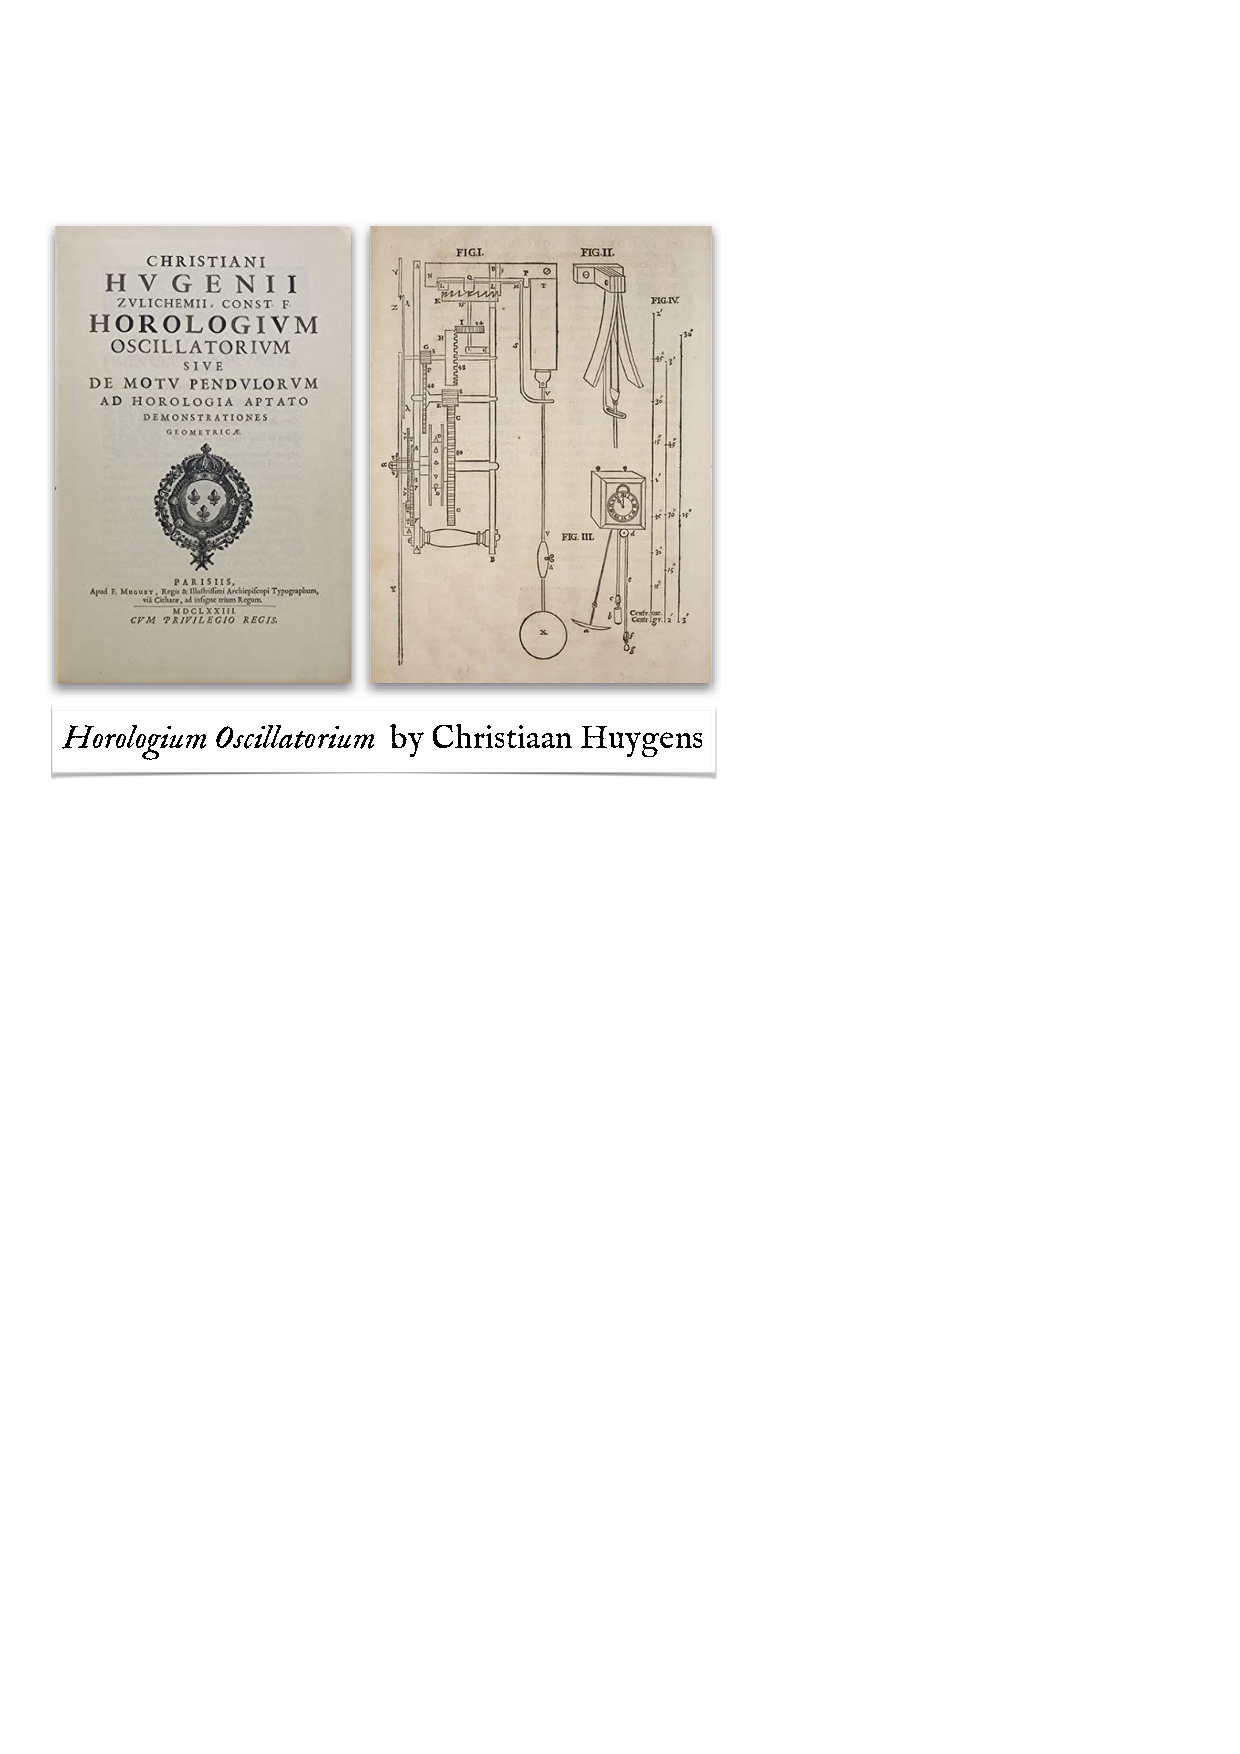
\includegraphics[width=.7\textwidth]{Figures/Horologium.pdf}}
